\documentclass{standalone}
\usepackage{tikz}
\usetikzlibrary{through,calc, quotes,angles}

\begin{document}
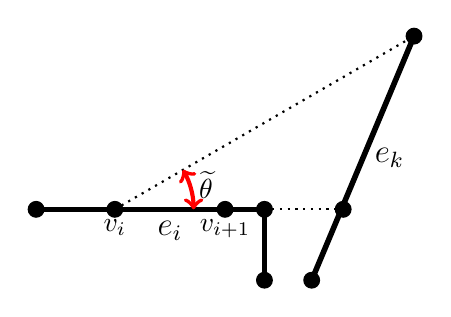
\begin{tikzpicture}
  \coordinate (A) at (-3, -4);
  \node at (A) [below] {$v_i$};
  \coordinate (B) at (-0.1, -4);
  \coordinate (C) at (0.8, -1.8);
  \coordinate (D) at (-1.1, -4);
  \coordinate (E) at (-1.1, -4.9);
  \coordinate (F) at (-0.5, -4.9);
  \coordinate (G) at (-1.6, -4);
  \coordinate (H) at (-4, -4);
  \node at (G) [below] {$v_{i+1}$};
  \draw [fill] (A) circle [radius=0.1];
  \draw [fill] (B) circle [radius=0.1];
  \draw [fill] (C) circle [radius=0.1];
  \draw [fill] (D) circle [radius=0.1];
  \draw [fill] (E) circle [radius=0.1];
  \draw [fill] (F) circle [radius=0.1];
  \draw [fill] (G) circle [radius=0.1];
  \draw [fill] (H) circle [radius=0.1];
  \draw [thick, line width=2pt](A) -- (G) node [midway, below, font = \large] {$e_i$};
  \draw [thick, line width=2pt](G) -- (D);
  \draw [thick, line width=2pt](H) -- (A);
  \draw [thick, line width=2pt](D) -- (E);
  \draw [thick, line width=2pt](C) -- (F) node [midway, right, font = \large] {$e_k$};
  \draw[thick, dotted] (A) -- (C);
  \draw[thick, dotted] (D) -- (B);
  \draw pic["$\widetilde{\theta}$",draw=red,<->,angle eccentricity=1.2,angle radius=1cm,line width=1.5pt] {angle=G--A--C};
\end{tikzpicture}
\end{document}
